% Created by tikzDevice version 0.12.3.1 on 2022-07-12 09:05:21
% !TEX encoding = UTF-8 Unicode
\documentclass{standalone}
\usepackage[table]{xcolor}
\usepackage{tikz}
\usepackage{fontspec}
\usepackage[abspath]{currfile}
\usepackage{booktabs}
\setmainfont[
Path={C:/Users/pgalvez/OneDrive - ine.gob.gt/Documentos/GitHub/CompendioGenero2023/Codigo/Fuentes/},,
BoldFont = OpenSans-CondBold.ttf ,
ItalicFont = OpenSans-CondLightItalic.ttf ,
BoldItalicFont = OpenSans-CondLightItalic.ttf
]{OpenSans-CondLight.ttf}
\newfontfamily\Bold{Open Sans Condensed Bold}
\newfontfamily\Sans{Open Sans}
\newfontfamily\SansBold{Open Sans Bold}
\newfontfamily\Italic{Open Sans Condensed Light Italic}
\newfontfamily\Logos{Latin Modern Roman}
\newfontfamily\Cinzel{Open Sans}

\usetikzlibrary{calc}
\usetikzlibrary{positioning}
\begin{document}
	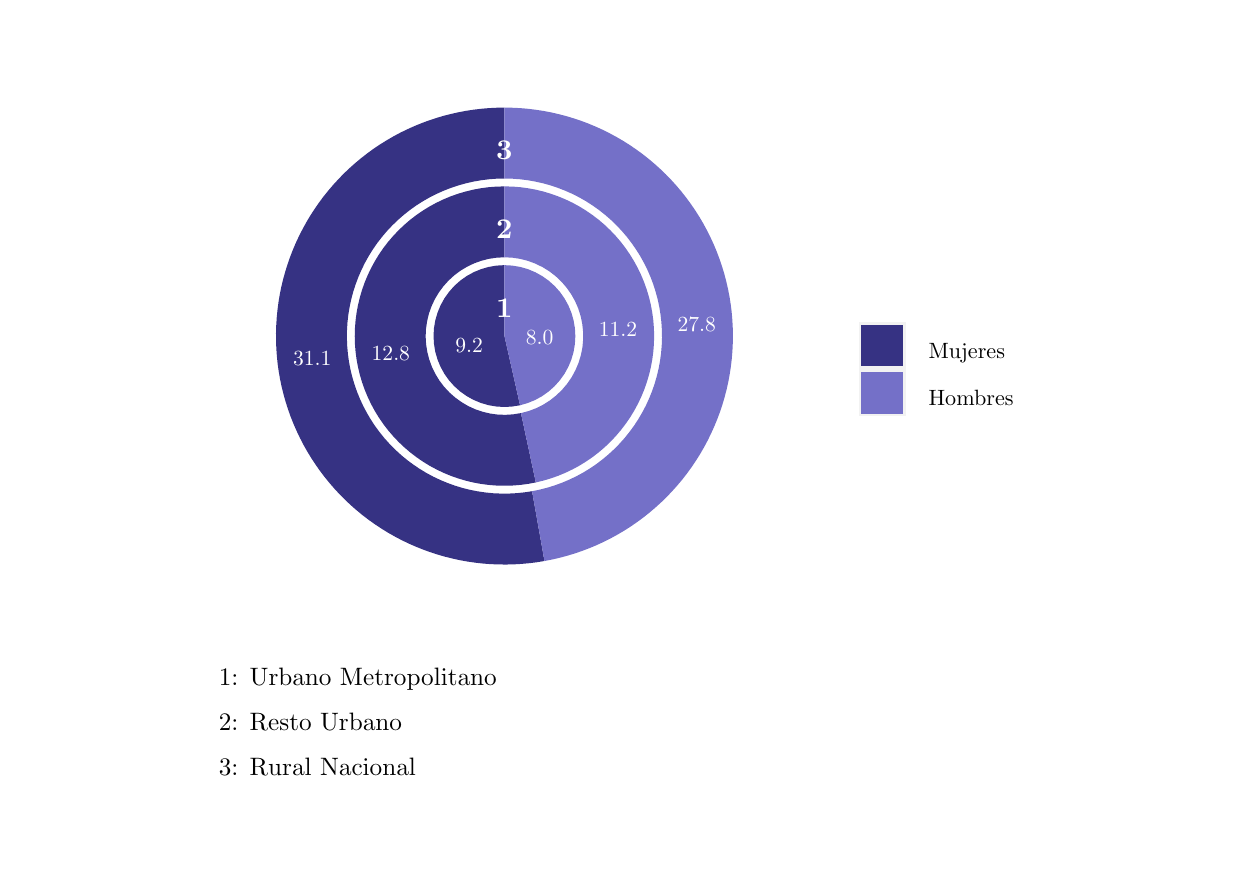
\begin{tikzpicture}[x=1pt,y=1pt, scale = 1.5]
		% Created by tikzDevice version 0.12.4 on 2023-05-05 09:28:13
% !TEX encoding = UTF-8 Unicode
\definecolor{fillColor}{RGB}{255,255,255}
\path[use as bounding box,fill=fillColor,fill opacity=0.00] (0,0) rectangle (289.08,198.74);
\begin{scope}
\path[clip] (  0.00,  0.00) rectangle (289.08,198.74);
\definecolor{drawColor}{RGB}{255,255,255}
\definecolor{fillColor}{RGB}{255,255,255}

\path[draw=drawColor,line width= 0.6pt,line join=round,line cap=round,fill=fillColor] ( 37.81,  0.00) rectangle (251.27,198.74);
\end{scope}
\begin{scope}
\path[clip] (  0.00,  0.00) rectangle (289.08,198.74);
\definecolor{fillColor}{RGB}{54,50,131}

\path[fill=fillColor] (114.85,124.45) --
	(114.85,126.34) --
	(114.85,128.24) --
	(114.85,130.14) --
	(114.85,132.04) --
	(114.85,133.93) --
	(114.85,135.83) --
	(114.85,137.73) --
	(114.85,139.63) --
	(114.85,141.53) --
	(112.94,141.42) --
	(111.06,141.10) --
	(109.22,140.57) --
	(107.45,139.84) --
	(105.77,138.91) --
	(104.21,137.81) --
	(102.78,136.53) --
	(101.51,135.10) --
	(100.40,133.54) --
	( 99.47,131.87) --
	( 98.74,130.10) --
	( 98.20,128.26) --
	( 97.88,126.38) --
	( 97.77,124.47) --
	( 97.88,122.56) --
	( 98.19,120.67) --
	( 98.72,118.83) --
	( 99.45,117.06) --
	(100.37,115.38) --
	(101.48,113.82) --
	(102.75,112.39) --
	(104.18,111.11) --
	(105.74,110.00) --
	(107.41,109.07) --
	(109.17,108.34) --
	(111.01,107.80) --
	(112.90,107.48) --
	(114.81,107.36) --
	(116.72,107.47) --
	(118.61,107.78) --
	(118.19,109.63) --
	(117.77,111.49) --
	(117.36,113.34) --
	(116.94,115.19) --
	(116.52,117.04) --
	(116.10,118.89) --
	(115.69,120.74) --
	(115.27,122.59) --
	(114.85,124.45) --
	(114.85,124.45) --
	cycle;

\path[fill=fillColor] (114.85,143.42) --
	(114.85,145.32) --
	(114.85,147.22) --
	(114.85,149.12) --
	(114.85,151.02) --
	(114.85,152.91) --
	(114.85,154.81) --
	(114.85,156.71) --
	(114.85,158.61) --
	(114.85,160.50) --
	(112.96,160.45) --
	(111.08,160.31) --
	(109.21,160.06) --
	(107.35,159.72) --
	(105.52,159.27) --
	(103.70,158.74) --
	(101.92,158.11) --
	(100.18,157.38) --
	( 98.48,156.57) --
	( 96.82,155.67) --
	( 95.21,154.68) --
	( 93.65,153.61) --
	( 92.15,152.46) --
	( 90.72,151.23) --
	( 89.35,149.93) --
	( 88.05,148.56) --
	( 86.82,147.13) --
	( 85.67,145.63) --
	( 84.60,144.07) --
	( 83.62,142.46) --
	( 82.72,140.80) --
	( 81.90,139.09) --
	( 81.18,137.35) --
	( 80.55,135.57) --
	( 80.02,133.76) --
	( 79.58,131.92) --
	( 79.23,130.06) --
	( 78.99,128.19) --
	( 78.84,126.31) --
	( 78.79,124.42) --
	( 78.84,122.53) --
	( 78.99,120.65) --
	( 79.24,118.77) --
	( 79.59,116.92) --
	( 80.03,115.08) --
	( 80.57,113.27) --
	( 81.20,111.49) --
	( 81.93,109.75) --
	( 82.74,108.04) --
	( 83.64,106.38) --
	( 84.63,104.77) --
	( 85.70,103.22) --
	( 86.85,101.72) --
	( 88.08,100.29) --
	( 89.38, 98.92) --
	( 90.76, 97.62) --
	( 92.19, 96.40) --
	( 93.69, 95.25) --
	( 95.25, 94.18) --
	( 96.86, 93.19) --
	( 98.52, 92.30) --
	(100.23, 91.48) --
	(101.98, 90.76) --
	(103.76, 90.14) --
	(105.57, 89.60) --
	(107.41, 89.16) --
	(109.26, 88.82) --
	(111.14, 88.58) --
	(113.02, 88.43) --
	(114.91, 88.39) --
	(116.80, 88.44) --
	(118.68, 88.59) --
	(120.55, 88.84) --
	(122.41, 89.19) --
	(122.01, 91.04) --
	(121.61, 92.90) --
	(121.21, 94.75) --
	(120.82, 96.61) --
	(120.42, 98.46) --
	(120.02,100.32) --
	(119.62,102.18) --
	(119.23,104.03) --
	(118.83,105.89) --
	(116.98,105.59) --
	(115.12,105.47) --
	(113.25,105.53) --
	(111.39,105.78) --
	(109.57,106.22) --
	(107.80,106.82) --
	(106.10,107.60) --
	(104.49,108.55) --
	(102.97,109.65) --
	(101.57,110.89) --
	(100.30,112.26) --
	( 99.17,113.75) --
	( 98.20,115.35) --
	( 97.38,117.03) --
	( 96.74,118.79) --
	( 96.27,120.60) --
	( 95.98,122.45) --
	( 95.87,124.31) --
	( 95.95,126.18) --
	( 96.22,128.03) --
	( 96.66,129.85) --
	( 97.28,131.62) --
	( 98.07,133.31) --
	( 99.03,134.92) --
	(100.14,136.43) --
	(101.39,137.82) --
	(102.77,139.08) --
	(104.27,140.20) --
	(105.87,141.16) --
	(107.56,141.97) --
	(109.32,142.60) --
	(111.13,143.06) --
	(112.98,143.33) --
	(114.85,143.42) --
	cycle;

\path[fill=fillColor] (114.85,162.40) --
	(114.85,164.30) --
	(114.85,166.20) --
	(114.85,168.10) --
	(114.85,169.99) --
	(114.85,171.89) --
	(114.85,173.79) --
	(114.85,175.69) --
	(114.85,177.59) --
	(114.85,179.48) --
	(112.99,179.45) --
	(111.13,179.36) --
	(109.27,179.20) --
	(107.42,178.98) --
	(105.58,178.70) --
	(103.75,178.35) --
	(101.93,177.94) --
	(100.13,177.48) --
	( 98.34,176.95) --
	( 96.57,176.36) --
	( 94.83,175.71) --
	( 93.10,175.00) --
	( 91.41,174.24) --
	( 89.73,173.42) --
	( 88.09,172.54) --
	( 86.48,171.60) --
	( 84.90,170.62) --
	( 83.35,169.58) --
	( 81.84,168.48) --
	( 80.37,167.34) --
	( 78.94,166.15) --
	( 77.55,164.91) --
	( 76.20,163.63) --
	( 74.90,162.29) --
	( 73.64,160.92) --
	( 72.43,159.50) --
	( 71.26,158.05) --
	( 70.15,156.55) --
	( 69.09,155.02) --
	( 68.08,153.46) --
	( 67.13,151.86) --
	( 66.23,150.22) --
	( 65.38,148.56) --
	( 64.59,146.88) --
	( 63.86,145.16) --
	( 63.19,143.42) --
	( 62.58,141.66) --
	( 62.03,139.89) --
	( 61.53,138.09) --
	( 61.10,136.28) --
	( 60.73,134.45) --
	( 60.42,132.61) --
	( 60.18,130.77) --
	( 60.00,128.91) --
	( 59.88,127.05) --
	( 59.82,125.19) --
	( 59.83,123.33) --
	( 59.90,121.46) --
	( 60.03,119.61) --
	( 60.22,117.75) --
	( 60.48,115.91) --
	( 60.80,114.07) --
	( 61.18,112.25) --
	( 61.63,110.44) --
	( 62.13,108.65) --
	( 62.70,106.87) --
	( 63.32,105.11) --
	( 64.01,103.38) --
	( 64.75,101.67) --
	( 65.55, 99.99) --
	( 66.40, 98.33) --
	( 67.31, 96.71) --
	( 68.28, 95.12) --
	( 69.30, 93.56) --
	( 70.37, 92.03) --
	( 71.49, 90.55) --
	( 72.67, 89.10) --
	( 73.89, 87.69) --
	( 75.15, 86.32) --
	( 76.47, 85.00) --
	( 77.82, 83.73) --
	( 79.22, 82.50) --
	( 80.66, 81.31) --
	( 82.14, 80.18) --
	( 83.66, 79.10) --
	( 85.21, 78.07) --
	( 86.80, 77.09) --
	( 88.42, 76.17) --
	( 90.07, 75.30) --
	( 91.74, 74.49) --
	( 93.45, 73.74) --
	( 95.18, 73.04) --
	( 96.93, 72.41) --
	( 98.70, 71.83) --
	(100.49, 71.31) --
	(102.30, 70.86) --
	(104.12, 70.46) --
	(105.95, 70.13) --
	(107.79, 69.86) --
	(109.65, 69.65) --
	(111.50, 69.51) --
	(113.36, 69.43) --
	(115.23, 69.41) --
	(117.09, 69.45) --
	(118.95, 69.56) --
	(120.81, 69.73) --
	(122.65, 69.96) --
	(124.49, 70.26) --
	(124.16, 72.13) --
	(123.83, 74.00) --
	(123.50, 75.86) --
	(123.16, 77.73) --
	(122.83, 79.60) --
	(122.50, 81.47) --
	(122.17, 83.34) --
	(121.83, 85.21) --
	(121.50, 87.07) --
	(119.64, 86.79) --
	(117.77, 86.60) --
	(115.90, 86.50) --
	(114.02, 86.50) --
	(112.14, 86.58) --
	(110.27, 86.77) --
	(108.41, 87.04) --
	(106.57, 87.40) --
	(104.74, 87.86) --
	(102.95, 88.40) --
	(101.18, 89.04) --
	( 99.44, 89.76) --
	( 97.74, 90.56) --
	( 96.09, 91.45) --
	( 94.48, 92.42) --
	( 92.92, 93.47) --
	( 91.41, 94.59) --
	( 89.96, 95.79) --
	( 88.57, 97.06) --
	( 87.25, 98.39) --
	( 85.99, 99.79) --
	( 84.81,101.25) --
	( 83.70,102.76) --
	( 82.66,104.33) --
	( 81.71,105.95) --
	( 80.83,107.61) --
	( 80.04,109.32) --
	( 79.33,111.06) --
	( 78.72,112.83) --
	( 78.18,114.64) --
	( 77.74,116.46) --
	( 77.39,118.31) --
	( 77.14,120.17) --
	( 76.97,122.04) --
	( 76.90,123.92) --
	( 76.92,125.80) --
	( 77.03,127.68) --
	( 77.24,129.55) --
	( 77.54,131.40) --
	( 77.93,133.24) --
	( 78.41,135.06) --
	( 78.98,136.85) --
	( 79.64,138.61) --
	( 80.38,140.33) --
	( 81.21,142.02) --
	( 82.12,143.66) --
	( 83.11,145.26) --
	( 84.18,146.81) --
	( 85.33,148.30) --
	( 86.54,149.73) --
	( 87.83,151.10) --
	( 89.18,152.40) --
	( 90.60,153.64) --
	( 92.07,154.81) --
	( 93.60,155.90) --
	( 95.19,156.91) --
	( 96.82,157.84) --
	( 98.49,158.69) --
	(100.21,159.46) --
	(101.96,160.14) --
	(103.74,160.74) --
	(105.55,161.24) --
	(107.38,161.66) --
	(109.23,161.98) --
	(111.10,162.22) --
	(112.97,162.36) --
	(114.85,162.40) --
	cycle;
\definecolor{fillColor}{RGB}{116,112,200}

\path[fill=fillColor] (114.85,124.45) --
	(115.27,122.59) --
	(115.69,120.74) --
	(116.10,118.89) --
	(116.52,117.04) --
	(116.94,115.19) --
	(117.36,113.34) --
	(117.77,111.49) --
	(118.19,109.63) --
	(118.61,107.78) --
	(120.45,108.31) --
	(122.23,109.04) --
	(123.91,109.96) --
	(125.47,111.07) --
	(126.90,112.34) --
	(128.18,113.77) --
	(129.30,115.33) --
	(130.23,117.01) --
	(130.97,118.77) --
	(131.50,120.62) --
	(131.82,122.51) --
	(131.93,124.42) --
	(131.83,126.33) --
	(131.51,128.22) --
	(130.98,130.07) --
	(130.25,131.84) --
	(129.32,133.52) --
	(128.22,135.08) --
	(126.94,136.51) --
	(125.51,137.79) --
	(123.95,138.90) --
	(122.27,139.83) --
	(120.50,140.57) --
	(118.66,141.10) --
	(116.77,141.42) --
	(114.85,141.53) --
	(114.85,139.63) --
	(114.85,137.73) --
	(114.85,135.83) --
	(114.85,133.93) --
	(114.85,132.04) --
	(114.85,130.14) --
	(114.85,128.24) --
	(114.85,126.34) --
	(114.85,124.45) --
	(114.85,124.45) --
	cycle;

\path[fill=fillColor] (118.83,105.89) --
	(119.23,104.03) --
	(119.62,102.18) --
	(120.02,100.32) --
	(120.42, 98.46) --
	(120.82, 96.61) --
	(121.21, 94.75) --
	(121.61, 92.90) --
	(122.01, 91.04) --
	(122.41, 89.19) --
	(124.24, 89.63) --
	(126.05, 90.17) --
	(127.83, 90.80) --
	(129.57, 91.53) --
	(131.27, 92.34) --
	(132.93, 93.24) --
	(134.53, 94.23) --
	(136.09, 95.30) --
	(137.58, 96.45) --
	(139.02, 97.68) --
	(140.38, 98.98) --
	(141.68,100.35) --
	(142.90,101.79) --
	(144.05,103.29) --
	(145.12,104.84) --
	(146.10,106.45) --
	(147.00,108.11) --
	(147.81,109.81) --
	(148.53,111.56) --
	(149.16,113.34) --
	(149.69,115.15) --
	(150.13,116.98) --
	(150.47,118.84) --
	(150.72,120.71) --
	(150.86,122.59) --
	(150.91,124.48) --
	(150.86,126.36) --
	(150.71,128.24) --
	(150.46,130.11) --
	(150.12,131.97) --
	(149.68,133.80) --
	(149.14,135.61) --
	(148.51,137.39) --
	(147.79,139.13) --
	(146.97,140.84) --
	(146.07,142.49) --
	(145.08,144.10) --
	(144.01,145.66) --
	(142.87,147.15) --
	(141.64,148.59) --
	(140.34,149.95) --
	(138.97,151.25) --
	(137.54,152.48) --
	(136.04,153.62) --
	(134.48,154.69) --
	(132.87,155.68) --
	(131.22,156.58) --
	(129.51,157.39) --
	(127.77,158.11) --
	(125.99,158.74) --
	(124.18,159.28) --
	(122.35,159.72) --
	(120.49,160.06) --
	(118.62,160.31) --
	(116.74,160.46) --
	(114.85,160.50) --
	(114.85,158.61) --
	(114.85,156.71) --
	(114.85,154.81) --
	(114.85,152.91) --
	(114.85,151.02) --
	(114.85,149.12) --
	(114.85,147.22) --
	(114.85,145.32) --
	(114.85,143.42) --
	(116.77,143.33) --
	(118.66,143.04) --
	(120.52,142.56) --
	(122.32,141.89) --
	(124.04,141.05) --
	(125.67,140.04) --
	(127.19,138.87) --
	(128.58,137.55) --
	(129.83,136.10) --
	(130.93,134.53) --
	(131.87,132.86) --
	(132.63,131.10) --
	(133.21,129.27) --
	(133.60,127.39) --
	(133.80,125.49) --
	(133.81,123.57) --
	(133.63,121.66) --
	(133.25,119.78) --
	(132.69,117.95) --
	(131.94,116.19) --
	(131.02,114.50) --
	(129.93,112.92) --
	(128.69,111.46) --
	(127.31,110.13) --
	(125.81,108.95) --
	(124.19,107.92) --
	(122.47,107.06) --
	(120.68,106.38) --
	(118.83,105.89) --
	cycle;

\path[fill=fillColor] (121.50, 87.07) --
	(121.83, 85.21) --
	(122.17, 83.34) --
	(122.50, 81.47) --
	(122.83, 79.60) --
	(123.16, 77.73) --
	(123.50, 75.86) --
	(123.83, 74.00) --
	(124.16, 72.13) --
	(124.49, 70.26) --
	(126.34, 70.62) --
	(128.16, 71.04) --
	(129.98, 71.53) --
	(131.77, 72.07) --
	(133.54, 72.68) --
	(135.30, 73.35) --
	(137.03, 74.07) --
	(138.73, 74.86) --
	(140.41, 75.70) --
	(142.05, 76.60) --
	(143.67, 77.55) --
	(145.25, 78.56) --
	(146.80, 79.63) --
	(148.31, 80.74) --
	(149.78, 81.91) --
	(151.20, 83.12) --
	(152.59, 84.38) --
	(153.94, 85.69) --
	(155.23, 87.05) --
	(156.48, 88.44) --
	(157.69, 89.88) --
	(158.84, 91.36) --
	(159.94, 92.88) --
	(160.99, 94.44) --
	(161.99, 96.03) --
	(162.93, 97.65) --
	(163.81, 99.30) --
	(164.64,100.99) --
	(165.41,102.70) --
	(166.12,104.43) --
	(166.78,106.19) --
	(167.37,107.97) --
	(167.90,109.77) --
	(168.37,111.59) --
	(168.78,113.42) --
	(169.12,115.26) --
	(169.40,117.12) --
	(169.62,118.98) --
	(169.77,120.85) --
	(169.86,122.72) --
	(169.89,124.60) --
	(169.85,126.48) --
	(169.75,128.35) --
	(169.59,130.22) --
	(169.36,132.08) --
	(169.07,133.93) --
	(168.71,135.78) --
	(168.29,137.60) --
	(167.82,139.42) --
	(167.27,141.21) --
	(166.67,142.99) --
	(166.01,144.75) --
	(165.29,146.48) --
	(164.51,148.18) --
	(163.67,149.86) --
	(162.78,151.51) --
	(161.83,153.13) --
	(160.82,154.71) --
	(159.76,156.26) --
	(158.65,157.77) --
	(157.49,159.25) --
	(156.28,160.68) --
	(155.02,162.07) --
	(153.72,163.42) --
	(152.36,164.72) --
	(150.97,165.97) --
	(149.53,167.18) --
	(148.06,168.34) --
	(146.54,169.44) --
	(144.99,170.50) --
	(143.40,171.50) --
	(141.78,172.44) --
	(140.13,173.33) --
	(138.45,174.17) --
	(136.74,174.94) --
	(135.01,175.66) --
	(133.25,176.32) --
	(131.47,176.91) --
	(129.68,177.45) --
	(127.86,177.92) --
	(126.03,178.34) --
	(124.19,178.69) --
	(122.33,178.97) --
	(120.47,179.20) --
	(118.60,179.36) --
	(116.73,179.45) --
	(114.85,179.48) --
	(114.85,177.59) --
	(114.85,175.69) --
	(114.85,173.79) --
	(114.85,171.89) --
	(114.85,169.99) --
	(114.85,168.10) --
	(114.85,166.20) --
	(114.85,164.30) --
	(114.85,162.40) --
	(116.73,162.36) --
	(118.60,162.22) --
	(120.46,161.99) --
	(122.31,161.66) --
	(124.14,161.25) --
	(125.94,160.75) --
	(127.72,160.15) --
	(129.47,159.47) --
	(131.19,158.71) --
	(132.86,157.86) --
	(134.49,156.93) --
	(136.07,155.92) --
	(137.60,154.83) --
	(139.07,153.67) --
	(140.49,152.44) --
	(141.84,151.14) --
	(143.12,149.77) --
	(144.34,148.35) --
	(145.48,146.86) --
	(146.55,145.32) --
	(147.55,143.73) --
	(148.46,142.09) --
	(149.29,140.41) --
	(150.04,138.69) --
	(150.70,136.93) --
	(151.27,135.14) --
	(151.76,133.33) --
	(152.15,131.50) --
	(152.45,129.65) --
	(152.66,127.78) --
	(152.78,125.91) --
	(152.81,124.03) --
	(152.74,122.16) --
	(152.58,120.29) --
	(152.33,118.43) --
	(151.99,116.59) --
	(151.55,114.76) --
	(151.03,112.96) --
	(150.42,111.19) --
	(149.72,109.45) --
	(148.94,107.74) --
	(148.07,106.08) --
	(147.12,104.46) --
	(146.10,102.89) --
	(144.99,101.37) --
	(143.82, 99.91) --
	(142.57, 98.51) --
	(141.25, 97.17) --
	(139.87, 95.90) --
	(138.43, 94.70) --
	(136.94, 93.57) --
	(135.38, 92.52) --
	(133.78, 91.54) --
	(132.13, 90.65) --
	(130.44, 89.84) --
	(128.71, 89.11) --
	(126.95, 88.47) --
	(125.16, 87.91) --
	(123.34, 87.45) --
	(121.50, 87.07) --
	cycle;
\definecolor{drawColor}{RGB}{255,255,255}

\node[text=drawColor,anchor=base,inner sep=0pt, outer sep=0pt, scale=  0.78] at (106.36,120.47) {9.2};

\node[text=drawColor,anchor=base,inner sep=0pt, outer sep=0pt, scale=  0.78] at ( 87.49,118.51) {12.8};

\node[text=drawColor,anchor=base,inner sep=0pt, outer sep=0pt, scale=  0.78] at ( 68.54,117.32) {31.1};

\node[text=drawColor,anchor=base,inner sep=0pt, outer sep=0pt, scale=  0.78] at (123.34,122.36) {8.0};

\node[text=drawColor,anchor=base,inner sep=0pt, outer sep=0pt, scale=  0.78] at (142.22,124.31) {11.2};

\node[text=drawColor,anchor=base,inner sep=0pt, outer sep=0pt, scale=  0.78] at (161.17,125.50) {27.8};

\node[text=drawColor,anchor=base,inner sep=0pt, outer sep=0pt, scale=  1.03] at (114.85,128.94) {\bfseries 1};

\node[text=drawColor,anchor=base,inner sep=0pt, outer sep=0pt, scale=  1.03] at (114.85,147.92) {\bfseries 2};

\node[text=drawColor,anchor=base,inner sep=0pt, outer sep=0pt, scale=  1.03] at (114.85,166.90) {\bfseries 3};
\end{scope}
\begin{scope}
\path[clip] (  0.00,  0.00) rectangle (289.08,198.74);
\definecolor{fillColor}{RGB}{255,255,255}

\path[fill=fillColor] (194.65, 99.59) rectangle (245.77,149.30);
\end{scope}
\begin{scope}
\path[clip] (  0.00,  0.00) rectangle (289.08,198.74);
\definecolor{fillColor}{gray}{0.95}

\path[fill=fillColor] (200.15,116.47) rectangle (211.53,127.85);
\end{scope}
\begin{scope}
\path[clip] (  0.00,  0.00) rectangle (289.08,198.74);
\definecolor{fillColor}{RGB}{54,50,131}

\path[fill=fillColor] (200.81,117.13) rectangle (210.87,127.19);
\end{scope}
\begin{scope}
\path[clip] (  0.00,  0.00) rectangle (289.08,198.74);
\definecolor{fillColor}{gray}{0.95}

\path[fill=fillColor] (200.15,105.09) rectangle (211.53,116.47);
\end{scope}
\begin{scope}
\path[clip] (  0.00,  0.00) rectangle (289.08,198.74);
\definecolor{fillColor}{RGB}{116,112,200}

\path[fill=fillColor] (200.81,105.75) rectangle (210.87,115.81);
\end{scope}
\begin{scope}
\path[clip] (  0.00,  0.00) rectangle (289.08,198.74);
\definecolor{drawColor}{RGB}{0,0,0}

\node[text=drawColor,anchor=base west,inner sep=0pt, outer sep=0pt, scale=  0.80] at (217.03,119.04) {Mujeres};
\end{scope}
\begin{scope}
\path[clip] (  0.00,  0.00) rectangle (289.08,198.74);
\definecolor{drawColor}{RGB}{0,0,0}

\node[text=drawColor,anchor=base west,inner sep=0pt, outer sep=0pt, scale=  0.80] at (217.03,107.65) {Hombres};
\end{scope}
\begin{scope}
\path[clip] (  0.00,  0.00) rectangle (289.08,198.74);
\definecolor{drawColor}{RGB}{0,0,0}

\node[text=drawColor,anchor=base west,inner sep=0pt, outer sep=0pt, scale=  0.91] at ( 46.06, 40.29) {1: Urbano Metropolitano};

\node[text=drawColor,anchor=base west,inner sep=0pt, outer sep=0pt, scale=  0.91] at ( 46.06, 29.49) {2: Resto Urbano};

\node[text=drawColor,anchor=base west,inner sep=0pt, outer sep=0pt, scale=  0.91] at ( 46.06, 18.69) {3: Rural Nacional};

\node[text=drawColor,anchor=base west,inner sep=0pt, outer sep=0pt, scale=  0.91] at ( 46.06,  7.89) {};
\end{scope}

	\end{tikzpicture}
\end{document}
